\documentclass{beamer}

\usetheme[displaysinglefooter,displaytocsection]{ISG}
%\usepackage{amsthm}
%\usepackage{xpatch}
%\usepackage{caption}

%\hypersetup{pdfpagemode=FullScreen}

\title{Example Beamer Presentation}
\subtitle{A Demonstration of the ISG Beamer Template}  
\author[R. Lee \& D. Hutchinson]{Robert Lee and Daniel Hutchinson}
\institute{Information Security Group,\\
Royal Holloway}

\begin{document}
\begin{frame}
\titlepage
\end{frame}

\begin{frame}\frametitle{Presentation Contents}
\tableofcontents
\end{frame}

\section{Available Footers}
\begin{frame}\frametitle{Split or Single?}
\begin{itemize}
	\item Two different footers are provided by the ISG style.  They are called split and single
	\item The single footer is the default and sets the footer as one solid orange bar
	\item The split footer divides the footer into two halves, orange and grey.  The title and authors are displayed on different sides of the orange/grey split.
	\item The footers are chosen by passing parameters when using the ISG theme, e.g.\ by \texttt{\textbackslash usetheme[displaysinglefooter]\{ISG\}} or \texttt{\textbackslash usetheme[displaysplitfooter]\{ISG\}}.
	\item Examples of each footer can be found in following slides.
\end{itemize}
\end{frame}

\begin{frame}\frametitle{Single Footer}
\begin{center}
	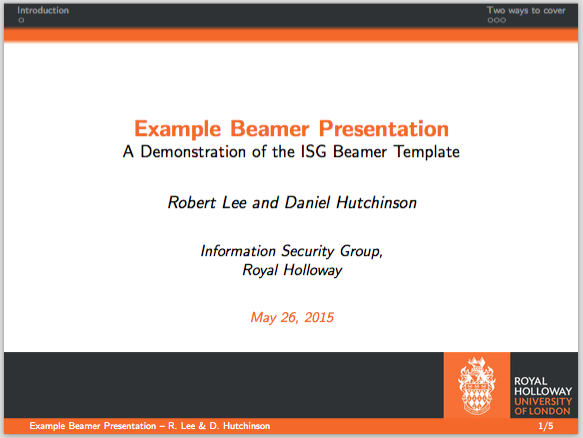
\includegraphics[scale=0.4]{graphics/single-footer.png}
\end{center}
\end{frame}

\begin{frame}\frametitle{Split Footer}
\begin{center}
	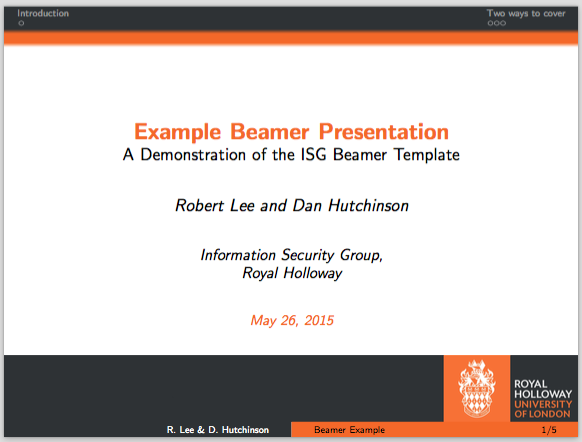
\includegraphics[scale=0.4]{graphics/split-footer.png}
\end{center}
\end{frame}

\section{Table of Contents on Section and Subsection}
\begin{frame}\frametitle{Showing progress through the presentation}
\begin{itemize}
\item The beamer style is also able to show a table of contents whenever a new section or subsection is begun.
\item These options are selected by passing the appropriate parameters when using the ISG theme.
\item E.g.\ \texttt{\textbackslash usetheme[displaytocsection]\{ISG\}} or \texttt{\textbackslash usetheme[displaytocsubsection]\{ISG\}}.
\item These can be used together with other options in the ISG style, e.g.\ this presentation uses the following\\ {\scriptsize\texttt{\textbackslash usetheme[displaysinglefooter, displaytocsection]\{ISG\}}}
\end{itemize}
\end{frame}

\setbeamercovered{invisible}
\section{Two ways to cover}
\begin{frame}\frametitle{Invisible Covering}
\begin{itemize}
\item{I'm the first item!}
\pause
\item{I was invisible!}
\pause
\item Invisible is selected by \texttt{\\setbeamercovered\{invisible\}}
\end{itemize}
\end{frame}


\setbeamercovered{transparent}
\begin{frame}\frametitle{Transparent covering}
\begin{itemize}
\item{I'm the first item!}
\pause
\item{I was transparent!}
\pause
\item Transparent is selected by \texttt{\\setbeamercovered\{transparent\}}
\end{itemize}
\end{frame}

\begin{frame}[allowframebreaks]
\frametitle{References}
\bibliography{presentation}
\end{frame}

\end{document}


